\textbf{Motivation.} In this section we describe the processes of Authentication and Authorization in the system.
It is worth to remember the meaning of Authentication and Authorization definitions.
Authentication -- is the process of ascertaining that somebody really is who they claim to be [\cite{burrows1989logic}].
Authorization refers to rules that determine who is allowed to do what [\cite{fagin1978authorization}].
For example, Adam may be authorized to create and delete databases, while Catherine is only authorized to read.
The two concepts are completely orthogonal and independent, but both are central to security design, and the
failure to get either one correct opens up the avenue to compromise.
In terms of web apps, very crudely speaking, authentication is when you check login credentials to see if you recognize
a user as logged in, and authorization is when you look up in your access control whether you allow the user to view,
edit, delete or create content.
Currently, there are two widely-known authentication methods, that are cookie authentication and JWT authentication.

\textbf{JWT Tokens.}
JSON Web Token or JWT is an open standard [\cite{jones2015rfc}] that defines a compact and self-contained way for securely
exchanging information between parties as a Javascript Object Notation (JSON) object [\cite{jones2015json}].
This information can be verified and trusted thanks to digital signature of the sender.
JSON Web Tokens could be signed using a secret with the HMAC,
stands for Hash-based Message Authentication Code algorithm [\cite{wang2004hmac}] or a public-private key pair using
the Rivest, Shamir and Adleman algorithm [RSA~\cite{wiener1990cryptanalysis}] or Elliptic Curve Digital Signature Algorithm
[ECDSA~\cite{johnson2001elliptic}].
Here are some scenarios JSON Web Tokens are useful in:

\begin{itemize}
    \item \textit{Authorization.} Is the most widely known scenario for using JWT\@.
    Once the user logs in, each further request will include the JWT to request header, allowing the user to access routes,
    services, and resources that are permitted with that token.
    Single Sign On is a feature that widely uses JWT nowadays, because of its small overhead and its ability to be easily
    used across different domains.
    Thanks to JWTs we are able to use Single Sign On feature, because of the JWTs' small overhead and ability to be
    used across different domains avoiding CORS errors.
    \item \textit{Information Exchange.} JSON Web Tokens may be used as secure way of communication.
    Because JWTs can be signed, it is simple to verify and identify the sender.
    Moreover, since that signature is calculated combining the header and the payload of the token, it is possible to verify
    that token has not been changed on the road.
\end{itemize}
JSON Web Token consists of the three parts separated by dots: Header, Payload, Signature.
Therefore, a JWT typically looks like
\begin{center}
    \begin{spverbatim}
        eyJhbGciOiJIUzI1NiIsInR5cCI6IkpXVCJ9.
        eyJqdGkiOiJmZDNjNjdjNS1jNmZmLTRhNWQtY
        TE2Ni05OGVjZTFiNzc1MmIiLCJyb2xlIjoiVX
        NlciIsIm5iZiI6MTYzMTU1MjQ5NiwiZXhwIjo
        xNjMxNTUyNzk2LCJpYXQiOjE2MzE1NTI0OTYs
        ImlzcyI6Imh0dHBzOi8vbWFuZ28tbWVzc2VuZ
        2VyLWFwcC5oZXJva3VhcHAuY29tIiwiYXVkIj
        oiaHR0cHM6Ly9tYW5nby1tZXNzZW5nZXItYXB
        wLmhlcm9rdWFwcC5jb20vYXBpIn0.
        locHt8ow1lFnGGZ_aFFvXI09dD4y1r594XQF2
        -6YxCw
    \end{spverbatim}
\end{center}
Let's discuss each part separately.
\begin{itemize}
    \item \textit{Header.} Typically, consists of two parts: the type of the token, and the signing algorithm
    being used, like \texttt{HMAC SHA256} or \texttt{RSA}.
    Example of header is as follows

    \begin{spverbatim}
    {
        "alg": "HS256",
        "typ": "JWT"
    }
    \end{spverbatim}

    After that, JSON is Base64 [\cite{josefsson2003rfc3548}] encoded to create the header part of the JWT\@.
    \item \textit{Payload.} The second part of the token is the payload with the entity claims.
    Claims are statements about the user and additional data.
    Claims are of the following types: registered, public and private claims.
    \begin{itemize}
        \item Registered claims.
        A set of predefined claims.
        Registered claims are not mandatory but recommended, to provide a set of useful and interoperable claims.
        For example, the following are registered claims
        \texttt{iss} stands for issuer,
        \texttt{exp} stands for expiration time,
        \texttt{sub} stands for subject,
        \texttt{aud} stands for audience,
        and \href{https://tools.ietf.org/html/rfc7519#section-4.1}{others}.
        The claim names are only three characters long to maintain the compactness of the JWT\@.
        \item Public claims.
        These claims can be defined freely.
        In order to avoid collisions public claims should be defined in the
        \href{https://www.iana.org/assignments/jwt/jwt.xhtml}{IANA JSON Web Token Registry}
        or to be defined in a form of URI which contains a collision resistant namespace.
        \item Private claims. These claims are the claims which can be created manually in order to share
        the information between the parties.
    \end{itemize}
    An example payload could be:

    \begin{spverbatim}
    {
        "sub": "10203040",
        "name": "Alice Fox",
        "approved": true
    }
    \end{spverbatim}

    The payload is then Base64 encoded to form the second part of the JSON Web Token.
    It is recommended to put secret information in payload or header only in encrypted form, since that Base64 is encoding
    only and can be read by anyone.
    \item \textit{Signature.} The signature part of the JWT is created combining the Base64 encoded
    header and payload using the specified in header algorithm.
    For instance, if the HMAC SHA256 algorithm is used, the signature will be created in the following way:

    \begin{spverbatim}
        HMACSHA256(
        base64UrlEncode(header) + "." +
        base64UrlEncode(payload),
        secret)
    \end{spverbatim}

    The signature is used to ensure that tokens wasn't changed during the exchange between parties,
    so-called Man in the middle attack.
    \item \textit{Conclusions.} JWT is three Base64 encoded strings separated by dots that can be
    used in authorization and information exchange over HTTP,
    JWTs are more compact related to XML-based standards like SAML\@.
\end{itemize}

As to the projects concerns, we should handle multiple client applications, e.g desktop,
web, mobile etc, therefore JWT authorization fits perfectly.

\textbf{JWT Authorization.} In authentication, when the user successfully logs in using their credentials,
a JSON Web Token will be returned.
Since tokens are credentials, great care must be taken to prevent security issues.
In general, you should not keep tokens longer than required.
You also should not store sensitive session data in browser storage due to lack of security.
Whenever the user wants to access a protected route or resource, the user agent should send the JWT,
typically in the Authorization header using the Bearer schema.
The content of the header should look like the following:
\begin{spverbatim}

    Authorization: Bearer <token>

\end{spverbatim}
This can be, in certain cases, a stateless authorization mechanism.
The server's protected routes will check for a valid JWT in the Authorization header, and if it's present,
the user will be allowed to access protected resources.
If the JWT contains the necessary data, the need to query the database for certain operations may be reduced,
though this may not always be the case.
If the token is sent in the Authorization header, Cross-Origin Resource Sharing (CORS) won't be an issue
as it doesn't use cookies.
Generally, the workflow is as follows
\begin{enumerate}
    \item User provides credentials in order to authenticate to the system.
    \item Server verifies user's authentication, fetches the login and password in database.
    \item If authentication is successful, server creates session then writes this session to the database.
    \item Server generates a pair of access JWT token and refresh token as GUID.
    \item Server sends to client access token and refresh token.
    \item Client saves the pair of access and refresh tokens.
    \item User requests resource using received token passed to the request header.
    \item The server check user's claims and proceeds or declines request.
\end{enumerate}

The eighth point is the authorization.
As a result, token stored on the client and used when it is necessary to authorize the requests.
When a hacker tries to replace the data in the header or payload the token will become invalid,
therefore the signature will not match the original values.
So, the hacker hasn't any possibility to generate a new signature since that encryption secret key stored on the server.
Access token in form of JWT is used for request authorization and for storing the additional information
about user like identifier, display name and others.
Refresh token in form of GUID issued by server based on successful authentication results and used
to get new access-refresh token pair.
Also, it is worth to add a few basic rules about JWT secure usage.
The lifetime of JWT should not be long since that stolen JWT cannot be revoked.
Randall Degges advices to follow the regulations [\cite{RDegges}]
\begin{itemize}
    \item JWT should have a short lifetime, since it cannot be revoked.
    \item JWT should be used in a single time, e.g.\ JWT per request.
\end{itemize}
However, extremely short lifetimes of the tokens would affect the overall performance of the system.
Therefore, we consider access token's lifetime to be 5 minutes and refresh token's 7 days.

For each request client preliminarily checks access token's lifetime.
If access token it expired, client sends request for updating a pair of access-refresh tokens.
For more confidence, we can update tokens a few seconds earlier.
That is, the case when the API receives an expired access token is practically excluded.
However, we are able to consider the case of interception of the request on \texttt{401UNAUTHORIZED} http status code.
The following diagram demonstrates the process of requesting the resource

\begin{figure}[H]
    \centering
    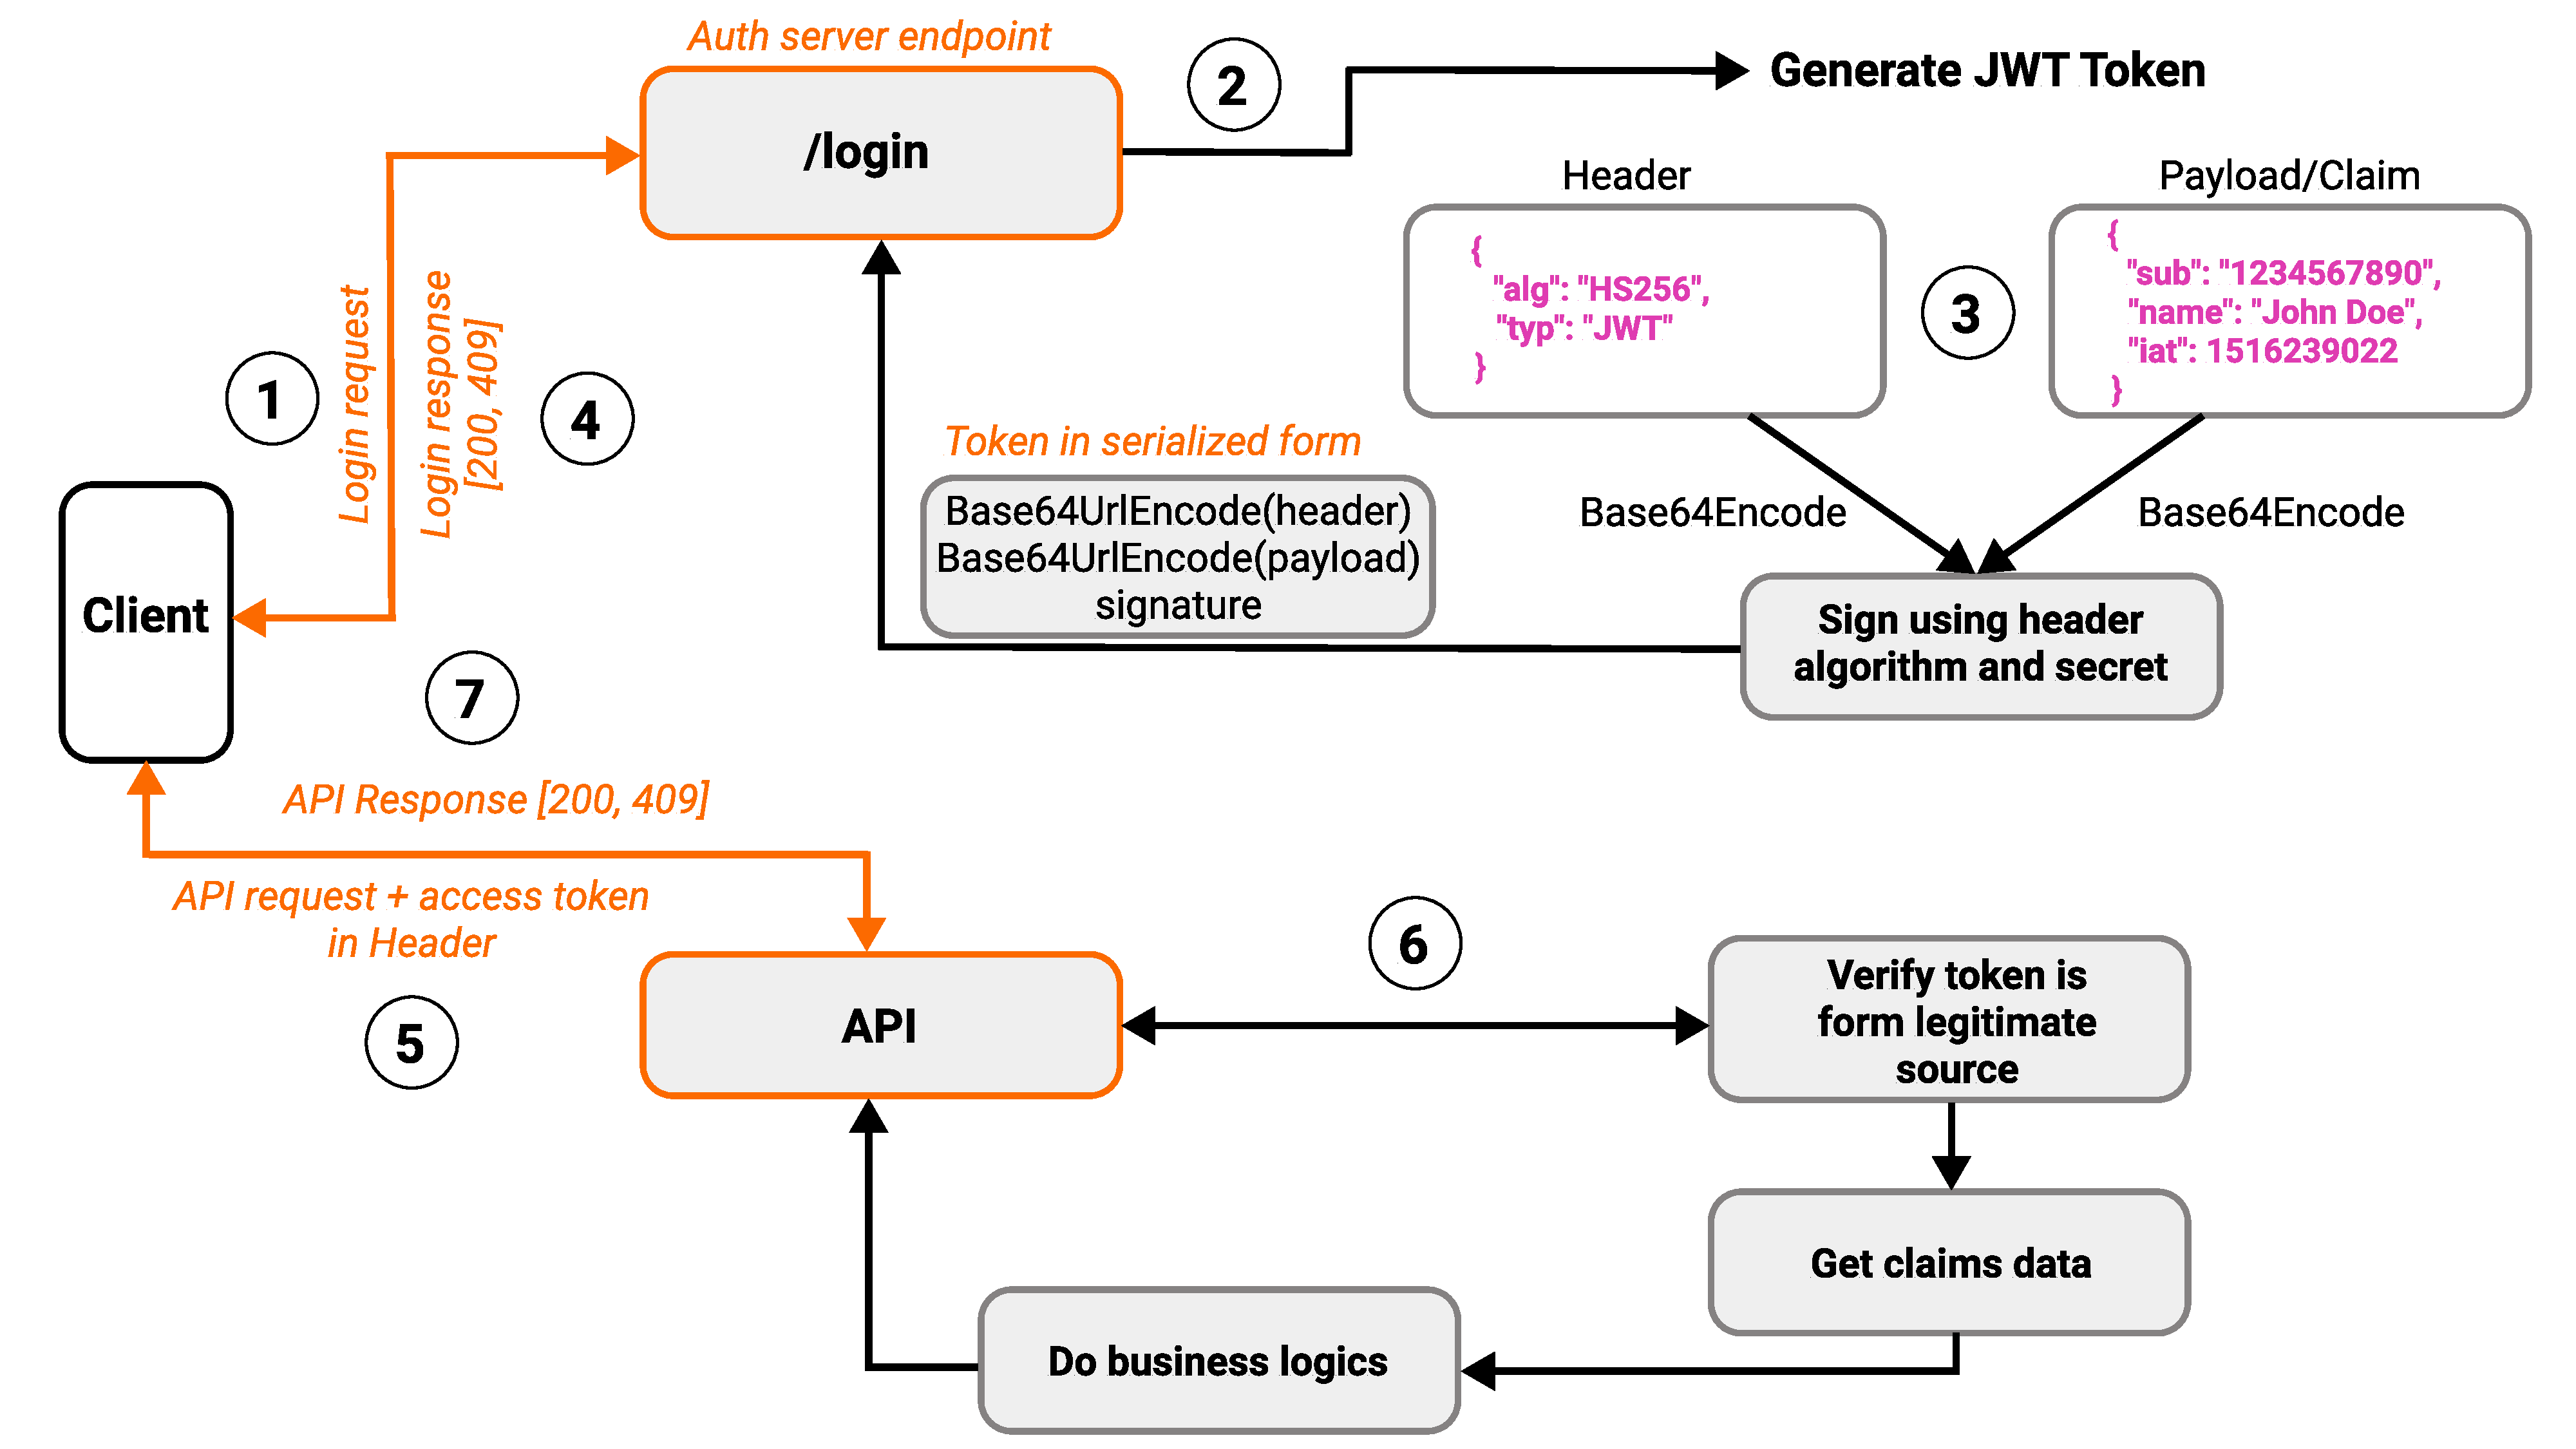
\includegraphics[width=1\textwidth]{Pictures/06_JWT_authorization_concept_diagram}
    \caption{JWT Authorization concept diagram.}\label{fig:figure3}
\end{figure}

By steps, the process is
\begin{itemize}
    \item \textbf{Step 1.} \textit{Client} application sends authentication request to
    the \textit{Auth server endpoint} provided user credentials in request body.
    \item \textbf{Step 2.} \textit{Auth server endpoint} responses to the \textit{Client} with the following
    HTTP response codes:
    \begin{itemize}
        \item \texttt{409CONFLICT}: Invalid credentials.
        \item \texttt{200SUCCESS}: Returns a pair of access and refresh tokens.
        \begin{itemize}
            \item \textbf{Step 3.} \textit{Auth server} generates a pair of access and refresh tokens
            \begin{itemize}
                \item \textit{Auth server} fetches user data and claims.
                \item \textit{Auth server} creates new session instance in database.
                \item \textit{Auth server} Base64 encodes access token's Header.
                \item \textit{Auth server} Base64 encodes access token's Payload.
                \item \textit{Auth server} generates access token's Signature using encoded token's
                Header and Payload signed by means of the \texttt{HMACSHA256} algorithm and secret.
            \end{itemize}
        \end{itemize}
    \end{itemize}
    \item \textbf{Step 4.} JWT access token in serialized form and refresh token in form of GUID are
    returned in response with \texttt{200SUCCESS} http status code to the \textit{Client} from the \textit{Auth server}.
    \item \textbf{Step 5.} \textit{Client} queries the \textit{API} providing access token as
    Bearer in request header.
    \item \textbf{Step 6.} \textit{API} validates the token claims in order to authorize user
    \begin{itemize}
        \item If authorized: \textit{API} handles the request, goes to \textbf{Step 7}.
        \item Otherwise: returns error with \texttt{401UNAUTHORIZED} http status code.
    \end{itemize}
    \item \textbf{Step 7.} \textit{} returns response with \texttt{200SUCCESS} or \texttt{409CONFLICT}
    http status codes to the client, according to business logic layer implementation.
\end{itemize}